%{{{Header
\documentclass[a4paper,10pt]{article}
\usepackage{anysize}
\marginsize{2cm}{2cm}{1cm}{1cm}
%\textwidth 6.0in \textheight = 664pt
\usepackage{xltxtra}
\usepackage{mathtools}
\usepackage{amsmath}
\usepackage{graphicx}
\usepackage{color}
\usepackage{xgreek}
\usepackage{fancyvrb}
\usepackage{minted}
\usepackage{listings}
\usepackage{hyperref}
\usepackage{enumitem}
\usepackage{framed}
\usepackage{relsize}
\usepackage{float}
\setmainfont[Mapping=TeX-text]{DejaVu Serif}
\newcommand{\tab}{\hspace*{3em}}

%\setmainfont{Arial}
%\setsansfont{FreeSans}
%\setmonofont{FreeMono}
\begin{document}
%\def\thesubsection {\alph{subsection}}
\renewcommand{\labelenumi}{\roman{enumi})}
\renewcommand{\labelenumii}{(\arabic{enumii})}

\begin{titlepage}
\begin{center}

\noindent\begin{minipage}[b]{.55\textwidth}
\begin{Large}
\emph{Εθνικό Μετσόβιο Πολυτεχνείο\\
Σχολή ΗΜ\&ΜΥ\\
Προγραμματιστικές Τεχνικές\\
2\textsuperscript{ο} εξάμηνο}
\end{Large}
\end{minipage}%
\begin{minipage}[b]{.45\textwidth}
     \centering
     
\includegraphics[scale=0.8]{title/ntua_logo}
\end{minipage}

\vspace{5cm}
\begin{huge}
\underline{Λύσεις Παλαιών Θεμάτων}
\end{huge}
\vfill

\begin{flushright}
\Large{Γερακάρης Βασίλης}\\
\large{\href{mailto:vgerak@gmail.com}{<vgerak@gmail.com>}}\\
\large{Α.Μ.: 03108092}\\
\end{flushright}
\vspace{1cm}

\end{center}
\end{titlepage}


%}}}

%{{{Σεπτ 2007
\section{Σεπτέμβριος 2007}
\setcounter{section}{1}

%{{{Q1: Execution time
\subsection{Θέμα 1 \textsuperscript{o}}
Κάθε βασική λειτουργία (tfetch, tstore, tC, tH, κ.λ.π.) = 1 μονάδα χρόνου, να
υπολογιστεί χρόνος εκτέλεσης και άνω ασυμπτωτικό όριο Ο() για τον παρακάτω
κώδικα:

\lstset{language=C, basicstyle=\footnotesize,
numbers=left,keywordstyle=\color{blue},commentstyle=\color{teal},stringstyle=\color{red}, frame=single}
\begin{lstlisting}
int K = 0;
for (int i = 0; i < n; ++i)
	for (int j = 1; j < n; ++j)
		++K;
\end{lstlisting}
%}}}

%{{{Q2: Stack pop & mult
\subsection{Θέμα 2 \textsuperscript{o}}
Θεωρώ ότι η isEmpty επιστρέφει 1 αν η στοίβα είναι άδεια, αλλιώς επιστρέφει 0.
Επιπλέον, η pop έχει ως τιμή επιστροφής την τιμή του στοιχείου που αφαιρείται.

\begin{lstlisting}
int product (stack s)
{
	int acc = 1;	//1 is the neutral element for multiplication
	while (isEmpty(s))
		acc *= pop(s);
	return acc
}
\end{lstlisting}

\begin{lstlisting}
//Easier to comprehend
int product (stack s)
{
	int acc = 1;
	int temp;
	while (isEmpty(s) != 1) {
		temp = pop(s);
		acc = acc * temp
	}
	return acc
}

\end{lstlisting}
%}}}

%{{{Q3: Recursion
\subsection{Θέμα 3 \textsuperscript{o}}
Cheat answer:
Δε θα τυπωθεί τίποτα, θα φάει syntax error στην \textit{"printf(“ΤΕΛΟΣ
\textbackslash{}n”;} \\

Serious answer:\\
A)
\begin{itemize}
	\item f(10)	-> τυπώνει 10, μπαίνει στο "n\%2 == 0" (c)
	\item f(5)	-> τυπώνει 5,  μπαίνει στο "else" (c)
	\item f(16)	-> τυπώνει 16,  μπαίνει στο (b)
	\item f(8)	-> τυπώνει 8,  μπαίνει στο (b)
	\item f(4)	-> τυπώνει 4,  μπαίνει στο (b)
	\item f(2)	-> τυπώνει 2,  μπαίνει στο (b)
	\item f(1)	-> τυπώνει 1,  μπαίνει στο "n==1", τυπώνει "ΤΕΛΟΣ" και τερματίζει
\end{itemize}

B) Θα τυπωθούν ακριβώς τα ίδια μηνύματα, με αντίστροφη σειρά:\\
ΤΕΛΟΣ, 1, 2, 4, 8, 16, 5, 10
%}}}

%{{{Q4: List Duplicates
\subsection{Θέμα 4 \textsuperscript{o}}

Υποθέτουμε ότι οι stdlib.h και string.h έχουν γίνει include στο αρχείο μας.\\
Υποθέτουμε επίσης ότι η δομή που χειριζόμαστε είναι η παρακάτω.

\begin{lstlisting}
struct node {
	char *word;
	struct node *next;
};
\end{lstlisting}

\begin{lstlisting}
struct node *remDupl(struct node *myList)
{
	struct node *ptr;
	struct node *temp;
	if (myList == NULL)
		return myList;	\\check if empty list
	ptr = myList;
	while (ptr->next != NULL) {
		if (strcmp(ptr->word, ptr->next->word) == 0) \{	\\if we find string match
			temp = ptr->next->next;	\\keep where the 2nd node points
			free(ptr->next);		\\delete node
			ptr->next = temp;		\\restore pointer
		} else
			ptr = ptr->next;		\\check next 2 nodes
	}
}
\end{lstlisting}
%}}}

%{{{Q5: Binary Tree
\subsection{Θέμα 5 \textsuperscript{o}}
A)\\
\begin{lstlisting}
int c = 0;	//global

int traverseCount(tree t)
{
	if(t == NULL)
		return 0;
	if(t->left != NULL && t->right != NULL)
		++c;
	traverseCount(t->left);
	traverseCount(t->right);
	return c;
}
\end{lstlisting}

B)
5 -> 4 -> 2 -> 8 -> 6 -> 7 -> 9
%}}}

%{{{Q6: BubbleSort
\subsection{Θέμα 6 \textsuperscript{o}}
Αρχικά : [2,1,4,1,6,8,3,5]\\
i = 7:

j = 1 : [1,2,4,1,6,8,3,5] (swap 1,2)

j = 2 : [1,2,4,1,6,8,3,5]

j = 3 : [1,2,1,4,6,8,3,5] (swap 1,4)

j = 4 : [1,2,1,4,6,8,3,5]

j = 5 : [1,2,1,4,6,8,3,5]

j = 6 : [1,2,1,4,6,3,8,5] (swap 3,8)

j = 7 : [1,2,1,4,6,3,5,\textbf{8}] (swap 5,8)
\\
i = 6:

j = 1 : [1,2,1,4,6,3,5,\textbf{8}]

j = 2 : [1,1,2,4,6,3,5,\textbf{8}] (swap 1,2)

j = 3 : [1,1,2,4,6,3,5,\textbf{8}]

j = 4 : [1,1,2,4,6,3,5,\textbf{8}]

j = 5 : [1,1,2,4,3,6,5,\textbf{8}] (swap 3,6)

j = 6 : [1,1,2,4,3,5,\textbf{6},\textbf{8}] (swap 5,6)
\\
i = 5:

j = 1 : [1,1,2,4,3,5,\textbf{6},\textbf{8}]

j = 2 : [1,1,2,4,3,5,\textbf{6},\textbf{8}]

j = 3 : [1,1,2,4,3,5,\textbf{6},\textbf{8}]

j = 4 : [1,1,2,3,4,5,\textbf{6},\textbf{8}] (swap 3,4)

j = 5 : [1,1,2,3,4,\textbf{5},\textbf{6},\textbf{8}]
\\
i = 4: Καμία αντιμετάθεση, ο πίνακας είναι ταξινομημένος.
%}}}

%{{{Q7: AVL Trees
\subsection{Θέμα 7 \textsuperscript{o}}
Εισαγωγή 1,4:
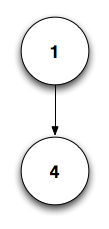
\includegraphics[scale=0.3]{files/im1_4.png}
Εισαγωγή 6 (rebalance):
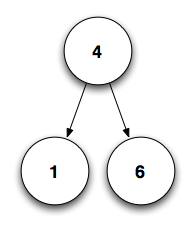
\includegraphics[scale=0.3]{files/im2_6.png}
Εισαγωγή 3:
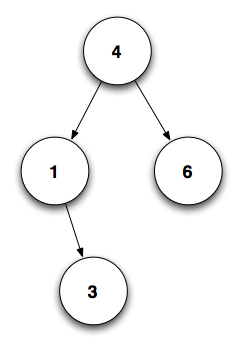
\includegraphics[scale=0.3]{files/im3_3.png}

Εισαγωγή 7:
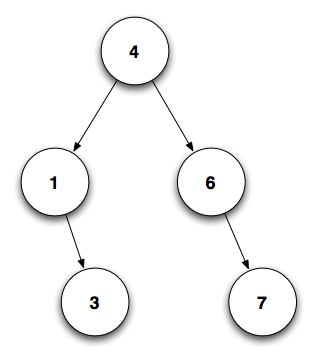
\includegraphics[scale=0.3]{files/im4_7.png}
Εισαγωγή 2 (rebalance):
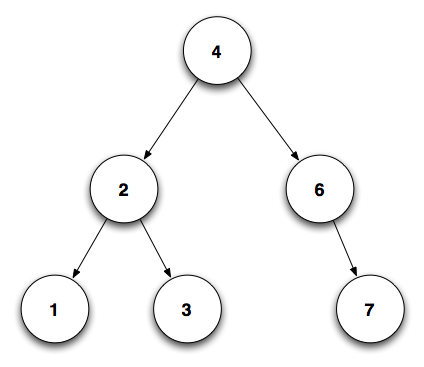
\includegraphics[scale=0.3]{files/im5_2.png}

Εισαγωγή 10 (rebalance):
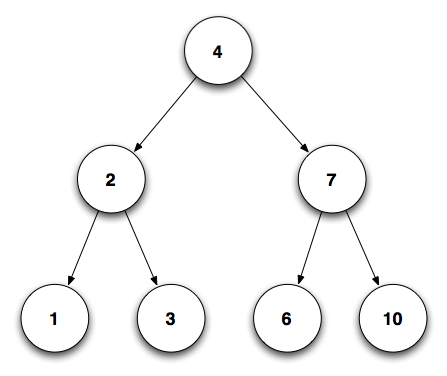
\includegraphics[scale=0.3]{files/im6_10.png}
%}}}

%}}}

%{{{Ιούλιος 2011
\section{Ιούλιος 2011}


%}}}


\end{document}
